% \iffalse
\let\negmedspace\undefined
\let\negthickspace\undefined
\documentclass[journal,12pt,twocolumn]{IEEEtran}
\usepackage{cite}
\usepackage{amsmath,amssymb,amsfonts,amsthm}
\usepackage{algorithmic}
\usepackage{graphicx}
\usepackage{textcomp}
\usepackage{xcolor}
\usepackage{txfonts}
\usepackage{listings}
\usepackage{enumitem}
\usepackage{mathtools}
\usepackage{gensymb}
\usepackage{comment}
\usepackage[breaklinks=true]{hyperref}
\usepackage{tkz-euclide} 
\usepackage{listings}
\usepackage{gvv}                                        
\def\inputGnumericTable{}                                 
\usepackage[latin1]{inputenc}                                
\usepackage{color}                                            
\usepackage{array}                                            
\usepackage{longtable}                                       
\usepackage{calc}                                             
\usepackage{multirow}                                         
\usepackage{hhline}                                           
\usepackage{ifthen}                                           
\usepackage{lscape}

\newtheorem{theorem}{Theorem}[section]
\newtheorem{problem}{Problem}
\newtheorem{proposition}{Proposition}[section]
\newtheorem{lemma}{Lemma}[section]
\newtheorem{corollary}[theorem]{Corollary}
\newtheorem{example}{Example}[section]
\newtheorem{definition}[problem]{Definition}
\newcommand{\BEQA}{\begin{eqnarray}}
\newcommand{\EEQA}{\end{eqnarray}}
\newcommand{\define}{\stackrel{\triangle}{=}}
\theoremstyle{remark}
\newtheorem{rem}{Remark}

\begin{document}

\bibliographystyle{IEEEtran}
\vspace{3cm}

\title{NCERT 11.9.5.30}
\author{EE23BTECH11043 - BHUVANESH SUNIL NEHETE$^{*}$% <-this % stops a space
}
\maketitle
\newpage
\bigskip

\renewcommand{\thefigure}{\theenumi}
\renewcommand{\thetable}{\theenumi}

\bibliographystyle{IEEEtran}

\section*{Question}
A man deposited Rs 10000 in a bank at the rate of 5\% simple interest anually. Find the amount in 15\textsuperscript{th} year since he deposited the amount and also calculate the total amount after 20 years.

\section*{Answer}
\fi
\begin{table}[h]
\renewcommand\thetable{1}
    \centering
    \begin{tabular}{|c|c|c|}
        \hline
        \textbf{Parameter} & \textbf{Value/Formula} & \textbf{description}\\
        \hline
        $x\brak{0}$ & Rs.10000 & Total amount deposited \\
        \hline
        $r$ & 5 & Rate of interest\\
        \hline
        $x\brak{n}$ & $\brak{x\brak{0} + nd}u\brak{n}$ & amount at the start of $\brak{n+1}\textsuperscript{th}$ year\\
        \hline
        $d$ & ? & common difference \\
        \hline
    \end{tabular}
    \caption{Input data}
    \label{tab:Input data}
\end{table}

\begin{align}
\text{Interest in one year} &= \frac{10000\times5\times1}{100}\\    
    d &= 500\label{eq1}
\end{align}
From \eqref{eq1} and \tabref{tab:Input data}:
    \begin{align}
        x(n) &= (10000 + 500n)u(n)
    \end{align}
From \eqref{eq:apz}
    \begin{align}
        X(z) &= \frac{10000}{1-z^{-1}} + \frac{500z^{-1}}{(1-z^{-1})^2} \quad |z|>1
    \end{align}
Amount in 15\textsuperscript{th} year is
    \begin{align}
        x(14) &= x(0) + 14\times d\\
        \implies x(14) &= 17000
    \end{align}
Total amount after 20 years is
    \begin{align}
        x(20) &= x(0) + 20\times 500\\
        \implies x(20) &= 20000
    \end{align}
    \begin{figure}[h]
    \renewcommand\thefigure{1}
        \centering
        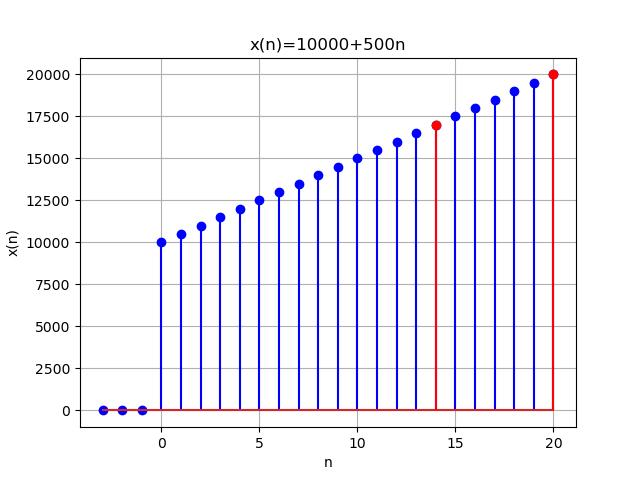
\includegraphics[width=1\linewidth]{ncert-maths/11/9/5/30/figs/p.jpeg}
        \caption{graph for $x(n) = 10000 + 500n$}
        \label{graph}
    \end{figure}

%\end{document}
